\chapter{Communicating Analyses and Building Data Products}
\label{chap:communication}
\chapterguide
  {You should be able to create statistical graphics, report uncertainty, validate models, and document limitations.}
  {design an evidence-first analytical narrative, choose an appropriate communication format, write concise executive summaries, distinguish reports from dashboards and notebooks, and plan monitoring for a deployed data product.}

\section{The final product is not the code}
Analytical code is essential for reproducibility, but stakeholders rarely make decisions by reading source files. The final product may be a report, dashboard, scheduled metric, model service, alert, or data table. Good data science connects the analytical artifact to a clear decision process without hiding uncertainty.

\begin{utpfig}[From analysis to action]{The communication layer translates technical evidence into an interpretable claim and then into an explicit decision or next step.}{fig:analysis-to-action}
\begin{tikzpicture}[x=\linewidth,y=1cm,
  stage/.style={draw=UTPBlue!70,fill=UTPPaleBlue,rounded corners=1.5mm,
    line width=0.6pt,text width=0.155\linewidth,minimum height=1.55cm,
    inner xsep=1.8mm,inner ysep=2mm,align=center,
    font=\scriptsize\color{UTPNavy}},
  flow/.style={-{Stealth[length=2mm,width=1.5mm]},
    line width=0.8pt,draw=UTPTeal}]
\node[stage] (data) at (0,0) {\textbf{Data}\\[4pt]
  Records with\\source and scope};
\node[stage] (analysis) at (0.205,0) {\textbf{Analysis}\\[4pt]
  Methods matched\\to the question};
\node[stage] (evidence) at (0.410,0) {\textbf{Evidence}\\[4pt]
  Results and\\diagnostics};
\node[stage] (claim) at (0.615,0) {\textbf{Claim}\\[4pt]
  Interpretation\\with uncertainty};
\node[stage,draw=UTPTeal!80,fill=UTPPaleTeal] (action) at (0.820,0)
  {\textbf{Decision}\\[4pt]
   Explicit action\\or next step};
\draw[flow] (data.east) -- (analysis.west);
\draw[flow] (analysis.east) -- (evidence.west);
\draw[flow] (evidence.east) -- (claim.west);
\draw[flow] (claim.east) -- (action.west);
\end{tikzpicture}
\end{utpfig}

\section{Start from the audience's decision}
A technical peer, an executive sponsor, and an operations team may need different views of the same analysis. The underlying evidence should remain consistent, but the level of detail and the action requested differ.

\begin{dstable}
\begin{tabularx}{\linewidth}{@{}p{2.8cm}p{3.8cm}X@{}}
\toprule
\rowcolor{DSPaleBlue!92}
Audience & Primary need & Useful content \\
\midrule
Technical reviewer & verify method & assumptions, code path, diagnostics, sensitivity checks \\
Decision maker & choose an action & main result, effect size, uncertainty, trade-offs, recommendation options \\
Operations team & execute consistently & thresholds, workflow, edge cases, escalation, monitoring \\
Future analyst & reproduce and extend & data version, scripts, environment, definitions, limitations \\
\bottomrule
\end{tabularx}
\end{dstable}

\section{An evidence-first story has a predictable structure}
Strong analytical communication is usually easier to follow when it answers five questions in order:
\begin{enumerate}
  \item What decision or question are we addressing?
  \item What data support the analysis, and what do they not cover?
  \item What is the main empirical pattern or model result?
  \item How uncertain or fragile is that result?
  \item What should happen next, and what should not be concluded?
\end{enumerate}

\begin{utpfig}[Evidence-first narrative]{A report should not force readers to reverse-engineer the question from a sequence of plots.}{fig:evidence-story}
\begin{tikzpicture}[x=\linewidth,y=1cm,
  stage/.style={draw=UTPBlue!70,fill=UTPPaleBlue,rounded corners=1.5mm,
    line width=0.6pt,text width=0.155\linewidth,minimum height=1.55cm,
    inner xsep=1.8mm,inner ysep=2mm,align=center,
    font=\scriptsize\color{UTPNavy}},
  flow/.style={-{Stealth[length=2mm,width=1.5mm]},
    line width=0.8pt,draw=UTPTeal}]
\node[stage] (q) at (0,0) {\textbf{Question}\\[4pt]
  Define the decision\\to be supported};
\node[stage] (d) at (0.205,0) {\textbf{Data and scope}\\[4pt]
  State sources\\and coverage};
\node[stage] (r) at (0.410,0) {\textbf{Result}\\[4pt]
  Present the main\\empirical finding};
\node[stage,draw=UTPOrange!80,fill=UTPPaleOrange] (u) at (0.615,0)
  {\textbf{Uncertainty}\\[4pt]
   Explain precision\\and limitations};
\node[stage,draw=UTPTeal!80,fill=UTPPaleTeal] (n) at (0.820,0)
  {\textbf{Next step}\\[4pt]
   Specify an action\\or further analysis};
\draw[flow] (q.east) -- (d.west);
\draw[flow] (d.east) -- (r.west);
\draw[flow] (r.east) -- (u.west);
\draw[flow] (u.east) -- (n.west);
\end{tikzpicture}
\end{utpfig}

\section{The executive summary should contain evidence, not adjectives}
A useful executive summary can often fit into one short paragraph:
\begin{enumerate}
  \item one sentence defining the question and scope;
  \item one sentence stating the main quantitative result;
  \item one sentence describing uncertainty or an important limitation;
  \item one sentence stating the decision implication or next analysis.
\end{enumerate}

Avoid unsupported words such as ``excellent'', ``dramatic'', or ``significant'' when a metric can communicate the result more precisely.

\begin{workedexample}
Weak: ``The new model performs extremely well and should be adopted.''

Stronger: ``Across five validation folds, accuracy ranged from 0.84 to 0.89. Sensitivity was lower for one small subgroup, so the model is suitable for further controlled evaluation but the threshold and subgroup behaviour should be reviewed before operational use.''
\end{workedexample}

\section{Uncertainty belongs in the main visual}
When the conclusion depends on an estimated quantity, uncertainty should not be hidden in a footnote. Confidence or prediction intervals, fold-to-fold variation, sensitivity analyses, or error bars can make the stability of the result visible.

\begin{utpfig}[Point estimates need their precision]{The intervals in this example make it immediately clear that some estimates are much less certain than others.}{fig:comm-uncertainty}
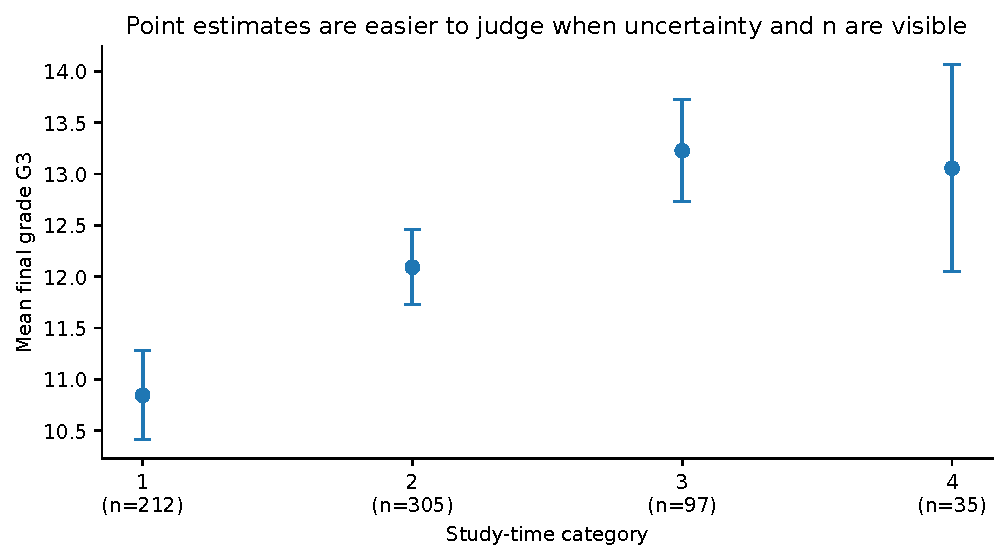
\includegraphics[width=0.78\linewidth]{figures_generated/comm_uncertainty.pdf}
\end{utpfig}

\section{Annotation directs attention without replacing evidence}
A title should state the question or conclusion the chart supports. Labels should identify important groups or thresholds. An annotation can explain an unusual point, a policy change, or a known data-quality event. The annotation should clarify the evidence rather than tell the reader what to believe despite the evidence.

\begin{utpfig}[A useful annotation connects a visual pattern to context]{The structure below separates measured evidence from contextual explanation.}{fig:annotation-structure}
\begin{tikzpicture}[x=\linewidth,y=1cm,
  card/.style={draw=UTPBlue!70,fill=UTPPaleBlue,rounded corners=1.5mm,
    line width=0.6pt,text width=0.35\linewidth,minimum height=1.45cm,
    inner xsep=3mm,inner ysep=2mm,align=center,
    font=\scriptsize\color{UTPNavy}},
  flow/.style={-{Stealth[length=2mm,width=1.5mm]},
    line width=0.8pt,draw=UTPTeal,rounded corners=1.5mm}]
\node[card,minimum height=3.55cm] (plot) at (0,0)
  {\textbf{Plot area}\\[5pt]
   Measured evidence\\
   and the observed pattern};
\node[card,draw=UTPOrange!80,fill=UTPPaleOrange] (ann) at (0.55,1.05)
  {\textbf{Annotation}\\[5pt]
   Context for a specific feature:\\
   ``Measurement process changed here''};
\node[card,draw=UTPTeal!80,fill=UTPPaleTeal] (cap) at (0.55,-1.05)
  {\textbf{Caption}\\[5pt]
   Definitions, data source,\\
   and relevant limitations};
\draw[flow,draw=UTPOrange!85!black] (ann.west) -- (0.275,1.05) --
  (0.275,0.65) -- ([yshift=6.5mm]plot.east);
\draw[flow] (cap.west) -- (0.275,-1.05) --
  (0.275,-0.65) -- ([yshift=-6.5mm]plot.east);
\end{tikzpicture}
\end{utpfig}

\section{Reports, notebooks, and dashboards serve different jobs}
A \term{notebook} is excellent for exploratory work and literate computation, but can become difficult to audit if execution order matters. A \term{report} is a stable narrative artifact for a defined question. A \term{dashboard} is useful when users need to inspect changing metrics repeatedly. None is universally superior.

\begin{dstable}
\begin{tabularx}{\linewidth}{@{}p{2.4cm}p{3.2cm}p{3.0cm}X@{}}
\toprule
\rowcolor{DSPaleBlue!92}
Format & Best for & Strength & Main risk \\
\midrule
Notebook & exploration and teaching & code + output together & hidden state, long narratives \\
Report & decision or study summary & stable argument & becomes stale if not regenerated \\
Dashboard & recurring monitoring & current metrics & context and uncertainty can disappear \\
Model/API service & automated decision support & consistent execution & failures can scale quickly \\
\bottomrule
\end{tabularx}
\end{dstable}

\section{A reproducible report has a dependency stack}
A report is reproducible only if the input data, code, software environment, and rendering process can be reconstructed.

\begin{utpfig}[Reproducibility stack]{Each layer depends on the layers below it. Saving only the final PDF preserves the result but not the process that produced it.}{fig:repro-stack}
\begin{tikzpicture}[node distance=0.24cm,
  layer/.style={draw=UTPBlue!70,fill=UTPPaleBlue,rounded corners=1.5mm,
    line width=0.6pt,minimum height=0.72cm,
    inner xsep=3mm,inner ysep=1.5mm,align=center,
    font=\scriptsize\bfseries\color{UTPNavy}},
  flow/.style={-{Stealth[length=1.6mm,width=1.3mm]},
    line width=0.8pt,draw=UTPTeal}]
\node[layer,text width=0.68\linewidth] (data) {Source data and version};
\node[layer,text width=0.60\linewidth,above=of data] (clean)
  {Cleaning and feature code};
\node[layer,text width=0.52\linewidth,above=of clean] (analysis)
  {Analysis and model code};
\node[layer,text width=0.44\linewidth,above=of analysis] (outputs)
  {Figures and tables};
\node[layer,text width=0.36\linewidth,above=of outputs,
  draw=UTPTeal!80,fill=UTPPaleTeal] (report) {Report};
\draw[flow] (data.north) -- (clean.south);
\draw[flow] (clean.north) -- (analysis.south);
\draw[flow] (analysis.north) -- (outputs.south);
\draw[flow] (outputs.north) -- (report.south);
\end{tikzpicture}
\end{utpfig}

\section{A data product continues after model fitting}
A deployed model is one component in a larger system. Inputs must be validated, features reproduced consistently, predictions logged, users supported, and performance monitored.

\begin{utpfig}[A minimal data-product architecture]{Training and serving should use compatible feature definitions. Monitoring closes the loop by comparing live behaviour with expectations from validation.}{fig:data-product-architecture}
\begin{tikzpicture}[x=\linewidth,y=1cm,
  stage/.style={draw=UTPBlue!70,fill=UTPPaleBlue,rounded corners=1.5mm,
    line width=0.6pt,text width=0.19\linewidth,minimum height=1.55cm,
    inner xsep=2.5mm,inner ysep=2mm,align=center,
    font=\scriptsize\color{UTPNavy}},
  flow/.style={-{Stealth[length=2mm,width=1.5mm]},
    line width=0.8pt,draw=UTPTeal,rounded corners=1.5mm},
  heading/.style={font=\scriptsize\bfseries\color{UTPNavy},
    anchor=west,inner sep=0pt}]
\node[heading] at (-0.11,2.20) {Training};
\node[stage] (train) at (0,1.05) {\textbf{Training data}\\[4pt]
  Versioned records\\and targets};
\node[stage] (pipe) at (0.25,1.05) {\textbf{Feature pipeline}\\[4pt]
  Learn and apply\\training transforms};
\node[stage] (model) at (0.50,1.05) {\textbf{Versioned model}\\[4pt]
  Fit and preserve\\model parameters};
\node[heading] at (-0.11,-0.25) {Serving};
\node[stage] (live) at (0,-1.40) {\textbf{Live input}\\[4pt]
  Validate incoming\\records};
\node[stage] (livepipe) at (0.25,-1.40) {\textbf{Feature pipeline}\\[4pt]
  Reuse definitions\\and fitted transforms};
\node[stage] (pred) at (0.50,-1.40) {\textbf{Prediction}\\[4pt]
  Apply the saved\\model};
\node[stage,draw=UTPTeal!80,fill=UTPPaleTeal] (mon) at (0.75,-1.40)
  {\textbf{Monitoring}\\[4pt]
   Log outputs\\and review behaviour};
\draw[flow] (train.east) -- (pipe.west);
\draw[flow] (pipe.east) -- (model.west);
\draw[flow] (live.east) -- (livepipe.west);
\draw[flow] (livepipe.east) -- (pred.west);
\draw[flow] (model.south) -- (pred.north);
\draw[flow] (pred.east) -- (mon.west);
\end{tikzpicture}
\end{utpfig}

\section{Distribution shift should be visible}
Even if code does not change, incoming data can. A feature may move because customer behaviour changes, sensors are recalibrated, a new market opens, or data collection changes.

\begin{utpfig}[Training and production distributions can diverge]{A shifted feature distribution does not prove that model accuracy has fallen, but it is a signal that the production environment no longer matches training conditions.}{fig:comm-drift}
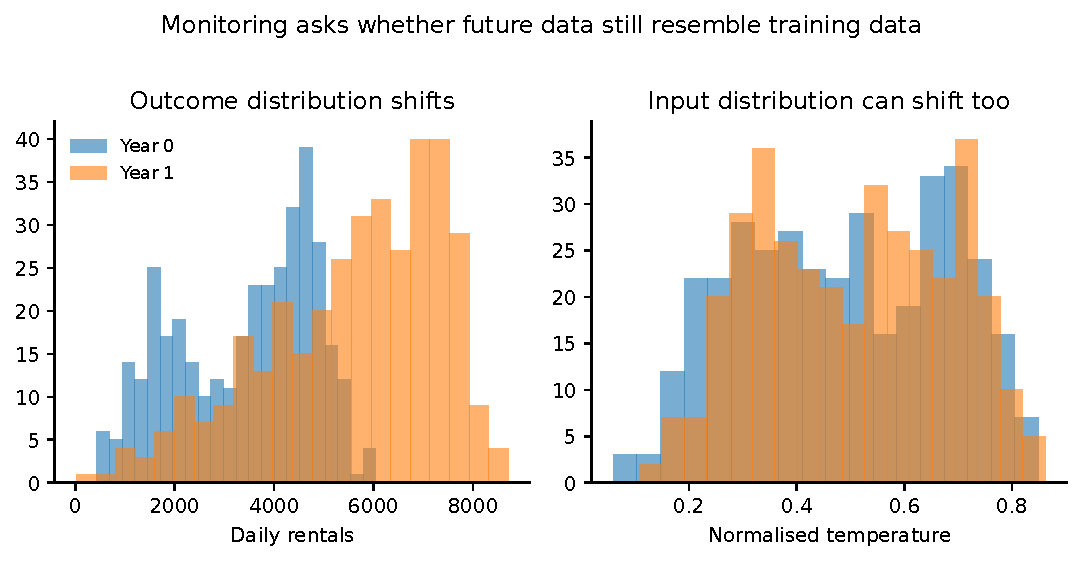
\includegraphics[width=0.82\linewidth]{figures_generated/comm_drift.pdf}
\end{utpfig}

Useful drift checks include changes in missingness, category frequencies, feature quantiles, prediction rates, and—when labels eventually arrive—performance metrics.

\section{Monitoring needs an action threshold}
Collecting dashboards without defining an action can create the appearance of control while problems accumulate. For each critical metric, specify an expected range, review threshold, owner, and response.

\begin{utpfig}[A monitoring metric becomes useful when a response is defined]{The example illustrates gradual degradation crossing a pre-specified review threshold. The threshold should trigger investigation, not automatic blame on the model.}{fig:comm-monitoring}
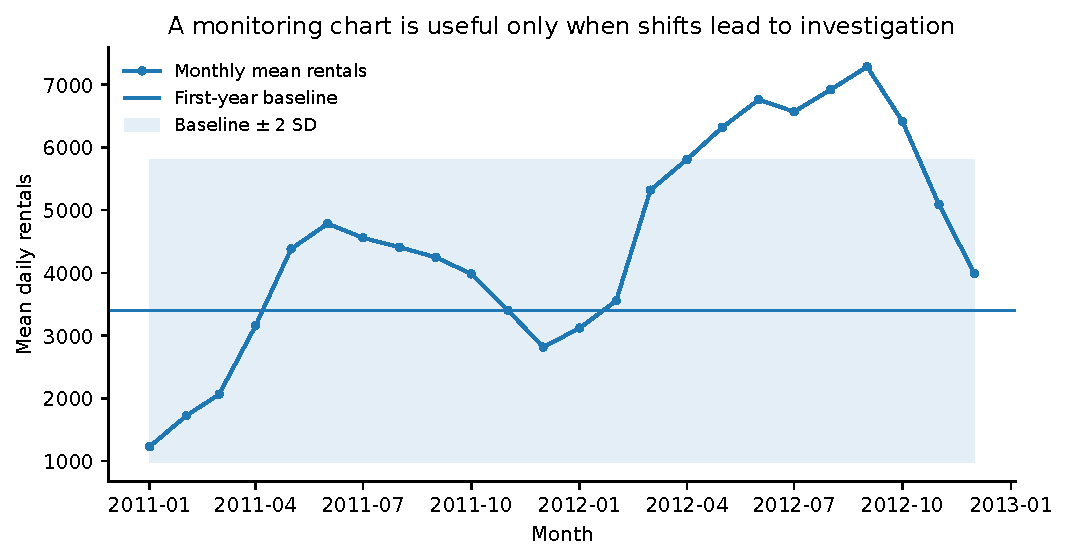
\includegraphics[width=0.83\linewidth]{figures_generated/comm_monitoring.pdf}
\end{utpfig}

\section{Model degradation has several possible causes}
A weaker live metric can arise from:
\begin{itemize}
  \item data-quality failures or changed units;
  \item population or feature distribution shift;
  \item changed relationships between features and outcomes;
  \item label delays or changed label definitions;
  \item operational changes downstream of the model;
  \item an implementation mismatch between training and serving.
\end{itemize}
Monitoring is therefore diagnosis, not merely score watching.

\section{Version the whole analytical decision}
A reproducible project records not only model weights but also data version, feature definitions, threshold, training code, metric definitions, and intended use. Two identical model coefficients can behave differently if the upstream feature pipeline or downstream threshold changed.

\begin{utpfig}[A deployable version is a bundle]{Treating the model as a bundle reduces the risk that a later system silently combines incompatible pieces.}{fig:model-bundle}
\begin{tikzpicture}[x=\linewidth,y=1cm,
  component/.style={draw=UTPBlue!70,fill=UTPPaleBlue,rounded corners=1.5mm,
    line width=0.6pt,text width=0.175\linewidth,minimum height=1.55cm,
    inner xsep=1.8mm,inner ysep=2mm,align=center,
    font=\scriptsize\color{UTPNavy}}]
\node[component] (schema) at (0,0) {\textbf{Data schema}\\[5pt]
  Version 3};
\node[component] (features) at (0.235,0) {\textbf{Feature code}\\[5pt]
  Version 7};
\node[component] (model) at (0.470,0) {\textbf{Model}\\[5pt]
  Version 5};
\node[component,draw=UTPOrange!80,fill=UTPPaleOrange] (policy) at (0.705,0)
  {\textbf{Threshold and}\\\textbf{policy}\\[5pt]
   Version 2};
\draw[draw=UTPTeal!80,line width=0.8pt,rounded corners=2mm]
  ([xshift=-3mm,yshift=4mm]schema.north west) rectangle
  ([xshift=3mm,yshift=-10mm]policy.south east);
\node[font=\scriptsize\bfseries\color{UTPTeal!85!black},align=center]
  at (0.3525,-1.35) {One reviewed release bundle};
\end{tikzpicture}
\end{utpfig}

\section{The capstone should read like a professional handoff}
The capstone in the next chapter should be understandable by someone who did not watch the analysis being produced. The reader should be able to identify the question, reproduce the evidence, see uncertainty, understand limitations, and know what additional data or validation would be needed next.

\begin{keyidea}
Communication is not decoration added after analysis. Choosing what to show, what uncertainty to preserve, and what action to connect to the result is part of the analytical design itself.
\end{keyidea}

\begin{quickcheck}
\begin{enumerate}
  \item How should a technical review differ from an executive summary while preserving the same evidence?
  \item When is a dashboard more appropriate than a static report?
  \item What is distribution shift, and why does it not automatically imply performance failure?
  \item Why should a monitoring metric have an owner and an action threshold?
  \item Which artifacts need to be versioned together for a deployable model?
\end{enumerate}
\end{quickcheck}

\section{Communicating evidence from different datasets}

The same reporting template should not flatten every problem into identical language. A regression model for Ames Housing, a rare-event fraud classifier, and a PCA of wine chemistry require different evidence in the main result.

\begin{dstable}
\begin{tabularx}{\linewidth}{@{}p{3.2cm}p{4.4cm}X@{}}
\toprule
\rowcolor{DSPaleBlue!92}
Analysis & Lead with & Do not hide \\
\midrule
Ames regression & holdout MAE/RMSE plus residual behaviour & expensive-home errors, missing predictors, nonlinearity \\
Fraud classification & prevalence, recall/precision, threshold, validation design & trivial accuracy baseline and false-positive cost \\
Student inference & effect size and uncertainty interval & observational design and plausible confounding \\
Mall clustering & cluster profiles in original units & sensitivity to scaling and chosen $k$ \\
Wine PCA & explained variance and loadings & standardisation choices and loss of information \\
\bottomrule
\end{tabularx}
\end{dstable}

This is the difference between a software report and an analytical report. The former lists functions that were run; the latter organises evidence around the decision, uncertainty, diagnostics, and limitations that a reader needs.

\begin{chapterrecap}
\begin{itemize}
  \item Analytical communication should start from the decision and preserve the evidence chain.
  \item Uncertainty and limitations belong in the main narrative, not only in technical appendices.
  \item Reports, notebooks, dashboards, and model services solve different communication and operational problems.
  \item Data products require reproducible feature pipelines, versioning, monitoring, and ownership after deployment.
  \item A strong capstone is a professional handoff that another analyst can inspect and reproduce.
\end{itemize}
\end{chapterrecap}
